\subsection{What is Azure Sphere}
Azure Sphere is a secured, high-level application platform with built-in communication and security features for internet-connected devices.

Azure Sphere introduces a new class of secured, connected, crossover MCU, which integrates real-time processing capabilities with a high-level 
operating system. Together with the application platform and enables product manufacturers to create secured, internet-connected device, so that
it can be updated, controlled, monitored, and maintained remotely. By embedding the MCU in a connected device, either alongside or in place of 
existing MCU(s), product manufacturers gain enhanced security, productivity, and opportunity. For example:
\begin{itemize}
    \item A secured application environment and authenticated connection can minimize the security risks from the spoofing, rogue software or denial of 
    service attacks.
    \item Software updates can be automatically deployed over the air to any connected device to provide new functionalities ,fix problems or counter 
    emerging methods of attacks, thus enhancing the productivity of support personnel.
    \item The cloud can diagnosing problems and designing new products over a secured connection, thus increasing the opportunity for product service, 
    positive customer interactions, and future development.
\end{itemize}

The Azure Sphere Security Service provides a safely and securely connect to the cloud and web. The service ensures that the device boots only with an authorized 
version of genuine, approved software. In addition, it provides a secured channel through which Microsoft can automatically download and install operating system 
updates to deployed devices in the field to mitigate security issues. Neither manufacturer nor end-user intervention is required, thus preventing a common security gap.

To read more about the Azure Sphere Security Service, please visit \href{https://docs.microsoft.com/en-us/azure-sphere/product-overview/azure-sphere-seven-properties}{Azure Sphere and the Seven Properties}


 \subsection{Hardware Specification}
 MT3620 features three user-accessible microcontroller cores, one application processor subsystem based on an ARM Cortex-A7 core which runs at up to 500MHz, 
 two general purpose ARM Cortex-M4F I/O subsystems, each of which runs at up to 200MHz. MT3620 were designed to support real-time requirements when interfacing 
 with a variety of on-chip peripherals including UART, I2C, SPI, I2S, and ADC. It has built-in security subsystem with its own dedicated CM4F core for secure 
 boot and secure system operation, dual-band 802.11a/b/g/n Wi-Fi.

 \begin{figure}[h]
     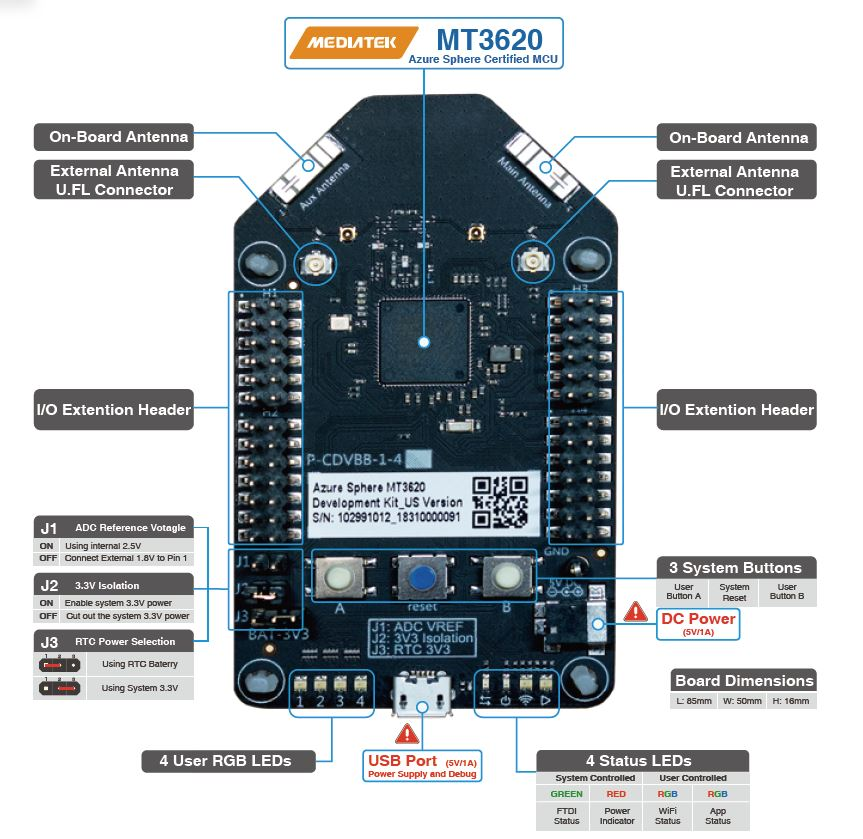
\includegraphics[scale=0.7]{HWDiagram.JPG}
 \end{figure}

 \begin{tabular}{c l} 
     MCU & 
     \begin{minipage}[t]{0.4\textwidth}
        \textbf{MT3620}
        \begin{itemize}
        \item 1 * ARM Cortex A7 core @500MHz , 4MB RAM
        \item ARM Cortex M4 core @200MHz , 64KB RAM
        \end{itemize}
      \end{minipage} \\
      \hline
     ICU & 
     \begin{minipage}[t]{0.4\textwidth}
        \textbf{4 * “ISU” serial interface which can be configured as:}
        \begin{itemize}
        \item I2C runs at up to 1MHz
        \item SPI runs at up to 40MHz
        \item UART runs at up to 3Mbps
        \end{itemize}
      \end{minipage} \\
      \hline
      Connectivity & 802.11 b/g/n Wi-Fi \\
      \hline
      I2S & 1 * I2S support slave and TDM slave mode \\
      \hline
      ADC & 4 * 12-bit ADC input I/O \\
      \hline
      RTC & 1 * RTC with CR2032 3V battery holder \\
      \hline
      USB & 1 * Micro USB port for power supply and debugging, 5V/1A \\
      \hline
      DC Jack 1* 5V/1A DC power jack \\
      \hline
      Operating Temperature & -40~85°C \\
      \hline
      Dimensions & L:85mm*W:50mm*H:16mm \\
      \hline
      Certification & CE / FCC / MIC / RoHS \\
 \end{tabular}

\subsection{Interface Headers}
The development board contains four banks of interface headers, labelled H1-H4, provide variety access of interfaces.The diagram shows 
the pin functions that are currently supported.
\begin{figure}[h]
    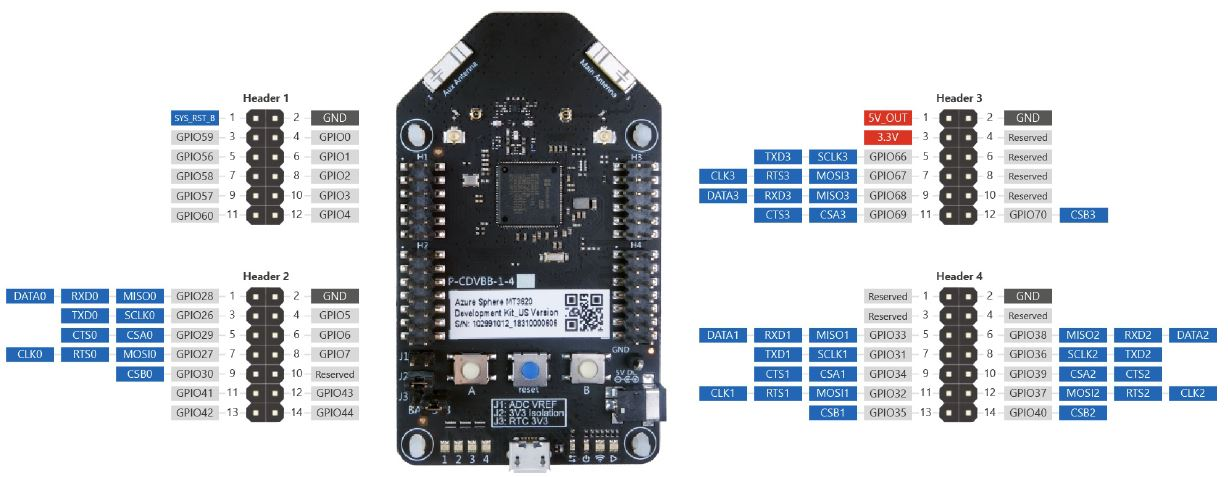
\includegraphics[width=\textwidth]{InterfaceHeaders.JPG}
\end{figure}
